% https://blogdoibre.fgv.br/posts/o-que-realmente-diz-o-relatorio-do-banco-central-sobre-spread-bancario
% ----
% Criação do documento com a classe abntex2
% ----
\documentclass[a4paper, article, 12pt, openany, oneside, english, brazil]{abntex2}

% ---
% Pacotes fundamentais
% ---
\usepackage{times}			    % Usa a fonte Latin Modern
\usepackage[T1]{fontenc}		% Seleção de códigos de fonte.
\usepackage[utf8]{inputenc}		% Codificação do documento (conversão automática dos acentos)
\usepackage{indentfirst}		% Indenta o primeiro parágrafo de cada seção.
\usepackage{color}		        % Controle das cores
\usepackage{graphicx}			% Inclusão de gráficos/figuras.
\usepackage{subcaption}			% Inclusão de sub-figuras.
\usepackage{microtype} 			% para melhorias de justificação
\usepackage{amsmath}			% Pacote matemático
\usepackage[brazil]{babel}

\autor{Phelipe Teles da Silva}
\titulo{Análise Quantitativa da Relação entre Spread e Concentração Bancária}
\data{2019}
\instituicao{Universidade Federal Rural do Rio de Janeiro}
\local{Seropédica, Rio de Janeiro}
\orientador[Orientadora:]{Débora Pimentel}

% ---
% Pacotes de citações
% ---
% \usepackage[brazilian,hyperpageref]{backref}	 % Paginas com as citações na bibliografia
\usepackage[alf]{abntex2cite}	                 % Citações padrão ABNT

\graphicspath{{../projeto/graficos/}}

\begin{document}

\section{Descrição das variáveis}

    Este capítulo pretende apresentar as relações teóricas entre a variável dependente e as variáveis independentes incluídas no modelo, assim como a evolução histórica das séries, abrangendo o período de março de 2011 a dezembro de 2018.

    Primeiro, o spread bancário. Trata-se, mais especificamente, da série 20786 do Sistema Gerenciador de Séries Temporais (SGS) do Banco Central do Brasil, intitulada "Spread médio das operações de crédito com recursos livres - Total", sendo a diferença, em pontos percentuais, entre a taxa média de empréstimo e de captação no mês. Por total, entende-se que ela aglutina operações de pessoas físicas e jurídicas, e por recursos livres, que exclui operações envolvendo taxas regulamentadas, lastreadas em recursos governamentais e afins.

    Na literatura, é o que se conhece por spread \textit{ex-ante}, porque é calculado antes do resultado, com base nas taxas estabelecidas pelos bancos, decisão em grande parte influenciada por suas expectativas. Por isso, esta taxa é mais volátil e mais sensível a mudanças macroeconômicas e risco percebido \cite[p.~226]{leal07}. Em contraste, o spread \textit{ex-post} é calculado com base na receita e despesa efetiva advinda da atividade de intermediação financeira \cite[p.~2]{almeida15}. 
    
    Na Fig. 1, salta à vista o aumento do spread a partir de 2014, após uma queda que se iniciou por volta de 2012 e que corresponde às políticas do primeiro governo de Dilma Rousseff com o intuito de reduzir o spread via aumento do portfólio de crédito dos bancos públicos, forçando uma queda pela competição das taxas de juros de empréstimos \cite[p.~1]{almeida15}. Porém, com a deterioração das condições macroeconômicas a partir de 2014, observamos a escalada do spread, seguido de um declínio iniciado em 2017 que veio com, entre outras coisas, a queda persistente da taxa SELIC a partir de então.

\begin{figure}[h]
  \centering
    \caption{Spread médio das operações de crédito com recursos livres - Total}
      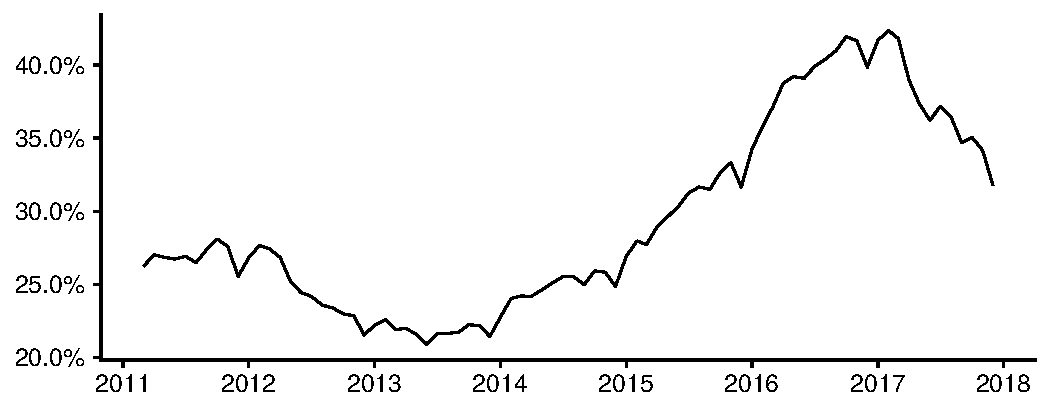
\includegraphics[width = \textwidth, scale=0.75]{Spread.pdf}
      \legend{Fonte: série 20786 do SGS. Elaboração própria}
      \label{spread}
\end{figure}
    
Este movimento da taxa SELIC pode ser visto na Fig. 2. A contraposição das duas séries sugere de imediato que elas são positivamente correlacionadas. De fato, é isso o que naturalmente se argumenta, porque uma taxa básica de juros mais elevada implica maior custo de oportunidade para a atividade de crédito, uma vez que aumenta a rentabilidade dos títulos públicos, tornando mais atrativa uma aplicação que já tem a vantagem de ser mais líquida e menos arriscada \cite[p.~372]{oliveira2007}. Por esta razão, é esperado um coeficiente positivo para a taxa básica de juros, pelo efeito custo de oportunidade. Na literatura empírica, não há divergências para essa estimativa, tendo a maior parte dos estudos encontrado a relação esperada \cite[p.~233-234]{leal07}.

\begin{figure}[h]
  \centering
    \caption{Taxa de juros - Selic acumulada no mês anualizada}
      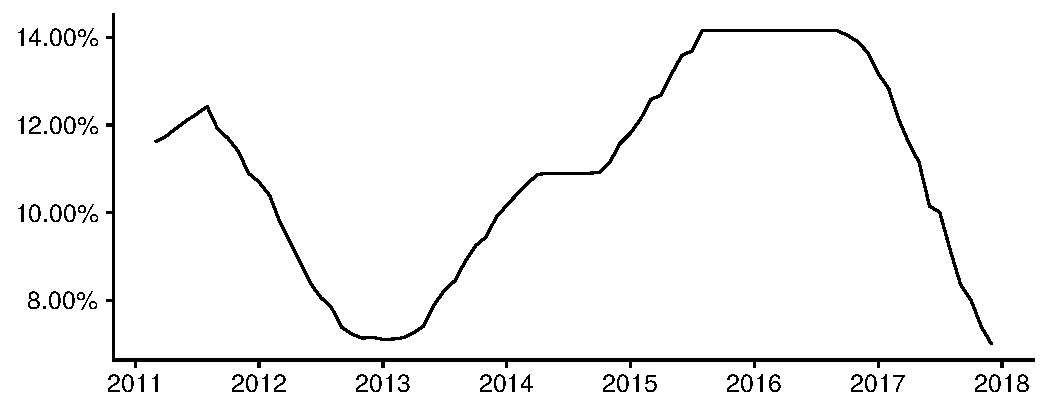
\includegraphics[width = \textwidth, scale=0.75]{Selic.pdf}
      \legend{Fonte: série 4189 do SGS. Elaboração própria}
      \label{selic}
\end{figure}
    
    Um padrão parecido pode ser observado na série da Inadimplência, na Fig. 3. A inadimplência passou a cair consideravelmente em 2012 para depois aumentar a partir de 2014 e 2015, com o advento da crise econômica. Não é surpreendente que haja uma correlação entre a Selic e a inadimplência, visto que um aumento da taxa básica de juros eleva o custo de captação, que é então repassado para o juros final, prejudicando a capacidade de pagamento \cite[p.~390]{oliveira2007}. A inclusão desta variável, portanto, serve para capturar o efeito do risco de crédito sobre o spread, \textit{ceteris paribus}.

\begin{figure}[t]
  \centering
    \caption{Inadimplência da carteira de crédito - Total}
      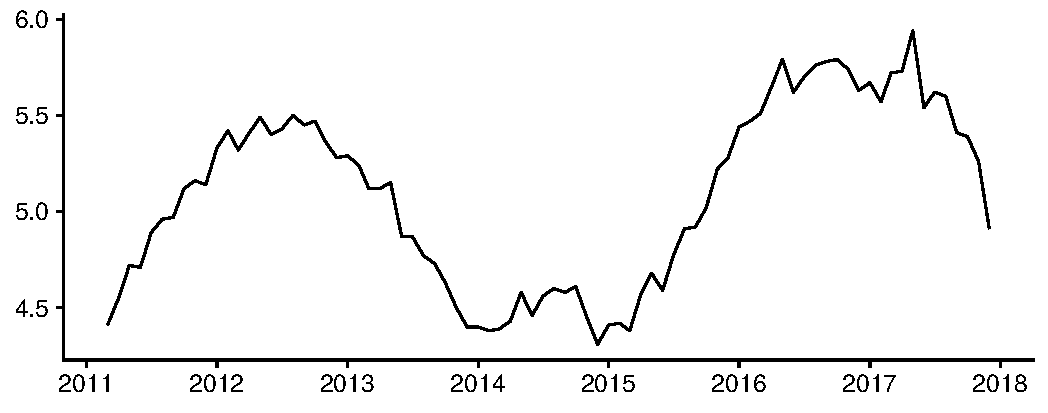
\includegraphics[width = \textwidth, scale=0.75]{Inadimplencia.pdf}
      \legend{Fonte: série 21085 do SGS. Elaboração própria}
      \label{inad}
\end{figure}
    
    A série de inflação escolhida foi o Índice Geral de Preços (IGP-DI), por ter apresentado resultados mais consistentes que o IPCA \cite[p.~66]{rocha09} e por ser mais abrangente \cite[p.~21]{afanasieff02}. A inclusão dessa variável se faz prudente porque sua variação pode influenciar a taxa básica de juros e a política de juros dos bancos, portanto o spread \cite[p.~14]{bignotto06}. O que se espera obter na estimação é um coeficiente positivo, indicando uma relação direta entre a inflação e o spread, devido ao fato de que em um ambiente econômico não sujeito à instabilidade dos preços os bancos não precisariam se proteger dela via spread. Se por um lado o efeito teórico esperado é claro, o que sairá na estimação é incerto, porque na literatura varia desde insignificante, como em \citeonline{oreiro}, a um sinal inesperado e significante, como em \citeonline{bignotto06} e \citeonline{afanasieff02}\footnote{Como possível causa, os autores indicam a apropriação de receita de senhoriagem com o spread \cite[p.~25]{afanasieff02}}.
    
\begin{figure}[h]
  \centering
    \caption{Índice Geral de Preços (IGP-DI)}
      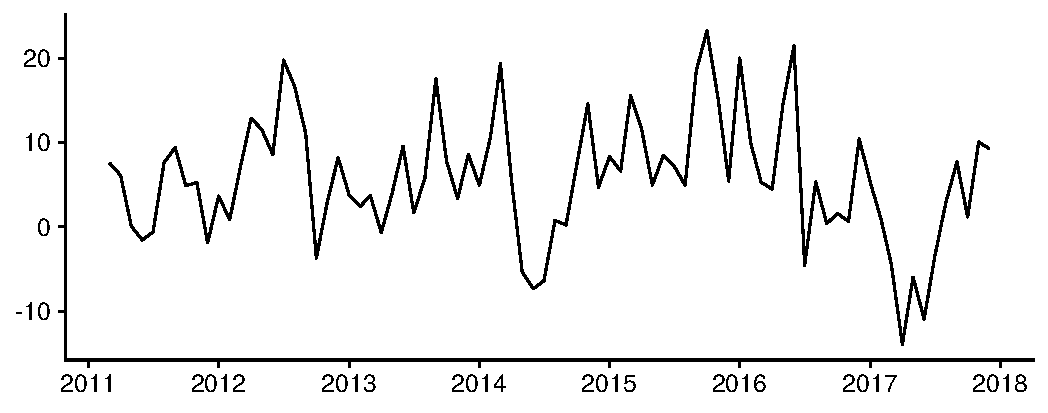
\includegraphics[width = \textwidth, scale=0.75]{IGP.pdf}
      \legend{Fonte: IPEA. Elaboração própria}
      \label{ipca}
\end{figure}
    
A série usada para capturar o efeito da atividade econômica sobre o spread é a Produção da indústria geral, calculada pelo IBGE como a variação percentual em relação ao mesmo período do ano anterior. Segundo \citeonline{oreiro}, o efeito desta variável sobre o spread é incerto, pois duas forças opostas entram em jogo: mais atividade econômica pode resultar em menor spread por reduzir o custo da concessão de crédito via aumento da escala de operação, mas também em maior spread porque mais pessoas demandarão crédito, o que pode elevar as taxas de empréstimo, o que por sua vez depende do poder de mercado dos bancos \citeonline[p.~626]{oreiro}. \citeonline{oreiro} encontram esta última relação na estimação, argumentando ter prevalecido o efeito poder de mercado. Os resultados não tem sido consistentes através dos estudos \cite[p.~236]{leal07}, mas de qualquer forma é considerada adequada sua inclusão como controle, evitando viés de variável omitida.
    
\begin{figure}[t]
  \centering
  \caption{Produção da indústria geral}
      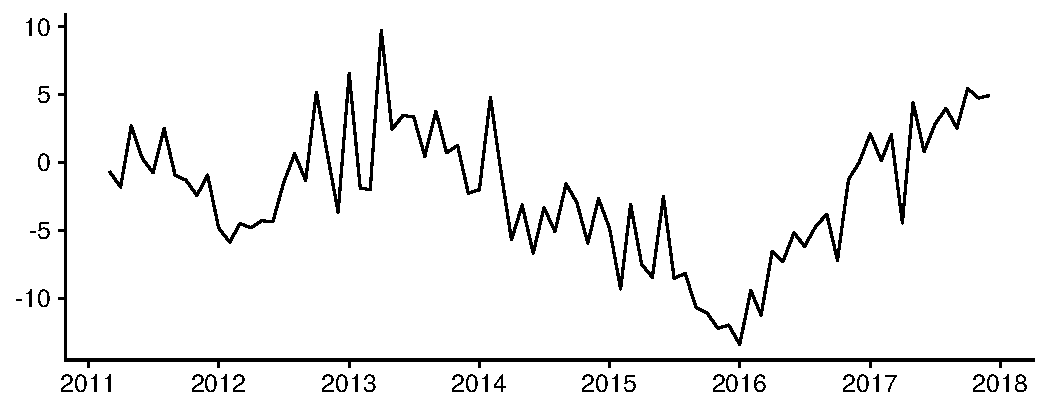
\includegraphics[width = \textwidth, scale=0.75]{ProducaoIndustrial_IPEADATA.pdf}
      \legend{Fonte: IBGE. Elaboração própria}
      \label{prodind}
\end{figure}
    
    Para as reservas compulsórias, será usada a série 1849 do SGS, divulgada mensalmente em milhares de unidades correntes. Para efeitos de apresentação, no entanto, os eixos estão em unidades de bilhões. O requerimento de reservas compulsórias faz parte do custo de intermediação dos bancos, sendo por isso pertinente a sua inclusão. Naturalmente, espera-se uma relação direta com o spread.

\begin{figure}[h]
  \centering
  \caption{Recolhimentos obrigatórios de instituições financeiras}
      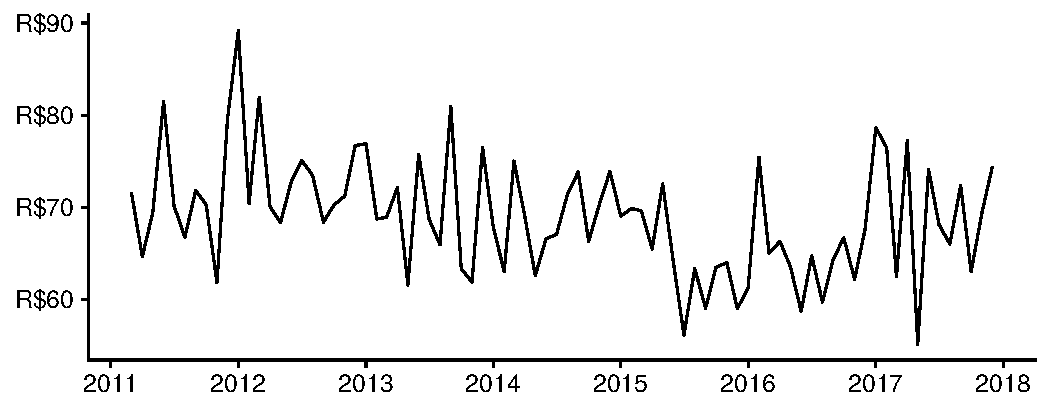
\includegraphics[width = \textwidth, scale=0.75]{Compulsorio.pdf}
      \legend{Fonte: série 1849 do SGS. Elaboração própria}
      \label{comp}
\end{figure}
    

\begin{figure}[h]
  \centering
  \caption{Índice de Herfindahl-Hirschmann - IHH}
      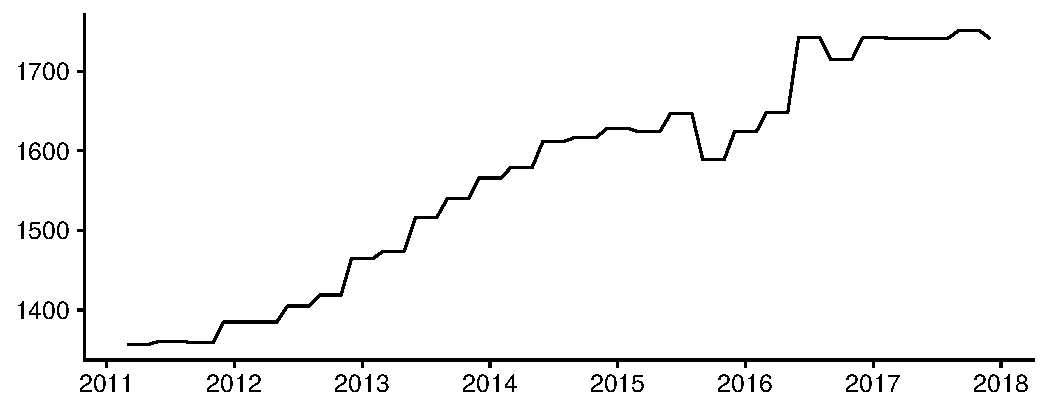
\includegraphics[width = \textwidth, scale=0.75]{IHH.pdf}
      \legend{Fonte: BCB. Elaboração própria}
      \label{comp}
\end{figure}
    
    Para a variável de concentração bancária, foi escolhido o índice de Herfindahl-Hirschmann, calculado pelo Banco Central do Brasil e divulgado no Anexo Estatístico do Relatório de Estabilidade Financeira, de abril de 2018. Os dados são trimestrais, por isso a necessidade de extrapolar os valores para os meses adjacentes. Como se sabe, este é um indicador do nível de concentração econômica em um mercado, obtido ao somar o quadrado das participações de cada instituição financeira no mercado considerado, que no nosso caso é o mercado de crédito. O BCB considera um IHH entre 0 e 1000 indicativo de baixa concentração, acima de 1000 e menor que 1800, de moderada concentração e acima de 1800 de alta concentração.

    Fica nítida a tendência de ascensão da concentração bancária, só refreada no final de 2015, voltando a crescer em seguida para depois permanecer estagnada, em um nível próximo do que é considerado uma concentração alta.

    No entanto, é preciso cautela na análise da concentração bancária como determinante do spread, já que a literatura sobre o assunto está longe de ser conclusiva \cite[p.~11]{reb2017}. De fato, como explicita \citeonline{reb2017}, há alta concentração bancária mesmo em países com um sistema financeiro considerado desenvolvido, isso porque esta indústria exige ganhos de escala e altos investimentos, o que está ligado à eficiência da intermediação financeira, que ajuda a reduzir o spread. Portanto, é possível que se encontre até mesmo uma relação inversa entre concentração e spread. 

    O relatório explica então que a variável relevante é a concorrência, que cresceu no período de 2000 a 2017 segundo o relatório \cite[p.~11]{reb2017}, ilustrando que maior concentração não implica necessariamente em menor concorrência.

    Dito isto, a inclusão desta variável é justificada pelo interessante aspecto teórico que ela representa. Apesar da dificuldade de predizer o sinal estimado, ainda é razoável que se espere um sinal positivo.

    Por fim, a \autoref{tab1} sumariza o que foi aqui discutido, listando cada variável e seus sinais esperados, além de algumas estatísticas descritivas.

    \begin{table}[t]
        \IBGEtab{\caption{Tabela de estatísticas descritivas}\label{tab1}}
        {
            \begin{tabular}
                {@{\extracolsep{5pt}}lccccc}
                \midrule
                \midrule
                Variável & \multicolumn{1}{c}{Média} & \multicolumn{1}{c}{Desvio Padrão} & \multicolumn{1}{c}{Mín.} & \multicolumn{1}{c}{Máx.} & \multicolumn{1}{c}{Sinal esperado} \\
                \midrule
                Spread & 29,33 & 6,51 & 20,89 & 42,34 &  \\
                Selic & 10,96 & 2,37 & 7,00 & 14,15 & + \\
                Inadimplência & 5,09 & 0,47 & 4,31 & 5,94 & + \\
                IGP-DI & 5,74 & 7,33 & $-$13,93 & 23,26 & + \\
                Atividade Econômica & $-$2,28 & 4,86 & $-$13,39 & 9,70 & +/- \\
                Compulsório (bilhões) & 68,92 & 6,32 & 55,13 & 89,17 & + \\
                IHH & 1.566,30 & 133,69 & 1.357 & 1.751 & + \\
                \midrule
            \end{tabular}
        }
        {\fonte{Elaboração própria.}\nota{Em sinal esperado, ``+'' indica um coeficiente positivo, ``-'', um negativo e ``0'' um não-significativo.}}
    \end{table}


\bibliography{../bibliografia}

\end{document}
